\documentclass[]{foi} 

\usepackage{graphicx}
\usepackage{array}
\usepackage{makecell}
\usepackage{booktabs}
\usepackage{caption}
\usepackage{float} 
\usepackage[utf8]{inputenc}
\usepackage{lipsum}
\usepackage{fvextra}
\usepackage{lineno}
\usepackage{csquotes}


\vrstaRada{\diplomski}

\title{Informativna platforma s inteligentnim asistentom o Erasmus+ iskustvu u \L\'{o}d\'{z}u}

\predmet{}

\author{Aleksandar Babić} 

\spolStudenta{\musko} 

\mentor{Bogdan Okreša Đurić}

\spolMentora{\musko} 

\titulaProfesora{doc.~dr.~sc.}

\godina{2025}
\mjesec{rujan}

\indeks{0016147642}

\smjer{Baze podataka i baze znanja}

\sazetak{Teoretski dio rada istražuje studiranje kao važan segment u životnom razdoblju pojedinca te se dotiče razmjene studenata u svrhu Erasmus+ studijskog boravka. 
Teoretski dio završava poglavljem posvećenim inteligentnim asistentima temeljenima na RAG (eng. Retrieval-Augmented Generation) tehnologiji.
Praktični dio rada obuhvaća izradu web-stranice s tematikom Erasmusa+ studijskog boravka i izradu inteligentnog asistenta, pri čemu će se iskoristiti postojeći jezični model. 
To podrazumijeva treniranje i prilagođavanje specifičnom skupu podataka, kako bi se osiguralo da inteligentni asistent odgovara upitima korisnika i pruža relevantne informacije.
}

\kljucneRijeci{Inteligentni asistent, RAG, web stranica, studiranje, Erasmus+, umjetna inteligencija.}

\acrodef{VAS}{višeagentni sustav}


\begin{document}

\maketitle

\tableofcontents

\makeatletter \def\@dotsep{4.5} \makeatother
\pagestyle{plain}



\chapter{Uvod}

Na početku rada obrađuje se pojam studiranja kao i svi aspekti koji se usko vežu uz njega. Poseban naglasak je stavljen na važnost studiranja u kontekstu osobnog razvoja, izgradnje karaktera
te stjecanja različitih znanja. U nastavku se detaljnije razmatra program Erasmus+, s ciljem približavanja njegovih mogućnosti i koristi. Glavni cilj je ukazati na izazove poput nedostatka interesa
za prijavu na Erasmus+ studijski boravak, prisutnog straha, nesigurnosti te neinformiranosti među studentima. 

Kao rješenje na ovaj problem izrađena je web stranica s inteligentnim asistentom koji je namijenjen da odgovori na specifične upite korisnika. Web stranica predstavlja sredstvo informiranja 
prvotno za sve studente koji dolaze u Łódź iz svojih država. Osim toga web stranica je naravno dostupna i namijenjena i za sve ostale zainteresirane posjetitelje. Web stranica se sastoji od 
početne stranice, stranice koja opisuje kratko Łódź, stranice koja prikazuje 15 najvećih grada Poljske i stranice na kojoj se nalazi forma. Forma je namijenjena za pitanja na koja nije mogao 
AI (eng. Artificial Inteligence) asistent odgovoriti. 

Za izradu AI modela odabrano je korištenje RAG (eng. Retrieval Augmenting Generation) gdje se uzima postojeći AI model i on se dotrenirava na specifičnom skupu podataka. 
Za takve potrebe pronađeno je nekoliko lokalnih web stranica koje opisuju život u Łódźu. Za potrebe treniranja razvijen je scraper koji dohvaća primarno tekstualni sadržaj s istih tih stranica
i sprema ih u JSON obliku. Naknadno su te JSON datoteke pročišćene i iskorištene za daljnje treniranje. Tijekom svoje Erasmus+ studentske mobilnosti imao sam prilike razgovarati s profesoricom na 
kolegiju Umjetna inteligencija, kojoj sam ukratko predstavio ideju svog diplomskog rada. Naknadno sam je zamolio da mi preporuči nekoliko korisnih stranica koje su vezane za Łódź. Budući da se profesorica rodila u Łódźu i tamo živi te radi cijeli život, smatrao sam da je upravo ona prava osoba kojoj se mogu obratiti
s pitanjem o korisnim izvorima informacija vezanima za život u Łódźu. 

Za tehnologije su odabrani: React (Java Script) za frontend, Python (za razvoj scrapera), NodeJS (Za razvoj servera na backendu), 
Python (za razvoj modela unutar Google Colab platforme). 

Prethodno ulomci uvode nas u temu s kojom se bavi ovaj rad, a to je „Informativna platforma s inteligentnim asistentom o Erasmus+ 
iskustvu u Łódźu“. Prvotna motivacija za proučavanje ove teme proizišla je iz Erasmus+ studijskog boravka u Łódźu (Poljska) u trajanju jednog semestra.



\chapter{Studiranje kao dio života pojedinca}

Važnost učenja se proteže kroz sve uzraste i faze života. Već od malih nogu školska djeca se potiču da marljivo uče jer to na neki način može odrediti njihov put u budućnosti.
Unutar ovog poglavlja više je vremena posvećeno studiranju kao važnom segmentu u životnom razdoblju pojedinca. U tom kontekstu visoko obrazovanje može napraviti razliku između uspješne osobe
i neuspjeha. Ulaganje u znanje je beskrajno i nikada ne prestaje i može se sagledati kao investicija u budućnost. Život bez obrazovanja je poput tijela bez duše, jer obrazovanje pojedincu donosi smisao, 
znanje i prilike koje oblikuju njegov osobni i profesionalni razvoj. Pomaže u razvoju kritičkog mišljenja, ima plemenit karakter i razvija vještine koje su potrebne za suočavanje sa svim životnim izazovima. 
Prema riječima stručnjaka iz škola u Bengaluru (Indija), studij je važan jer se koristi za ublažavanje kompleksnosti većine izazova s kojim se susretne pojedinac \cite{digital3602025studies}. 

%U nastavku su navedene prednosti učenja i obrazovanja: treniranje razmišljanja, treniranje kreativnosti, povećavnanje produktivnosti, 
%razumijavanje u teškim situacijama, jednostavnije zapošljavanje, treniranje fokusiranosti i koncentracije, uživanje u slobodnom vremenu, rješavanje složenijih problema, poboljšavanje pamćenja 
%poboljšavanje samopouzdanja, poboljšava vještina čitanja i pisanja \cite{digital3602025studies}.


\section{Odluka i benefiti}

Kod donošenja velikih odluka kao što je studiranje vrlo je bitno uzeti u obzir nekoliko čimbenika koji mogu oblikovati bolji pogled na razmišljanje o nečemu. Kada se razmišlja o tome da li krenuti
studirati ili ne, postoje ljudi koji govore da upisivanje fakulteta više nije presudno ni važno za uspjeh i da to može biti loša investicija ili da se može dobiti dobar posao bez odlaska na fakultet.
Primarni cilj ove sekcije nije zastupanje određene strane, već pružanje uvida u razloge zbog kojih bi upis na fakultet mogao biti dobra odluka. Započetak fakultet priprema radnu snagu za budući posao i može
dati značajnu prednost prilikom prijave za posao. Fakultetsko obrazovanje pokazuje poslodavcima da je osoba sposobna dovršiti dugoročni projekt, da je sposobna kritički razmišljati,
rješavati probleme i da je sposobna učiti nove stvari. Većina poslova danas zahtijeva barem neko fakultetsko iskustvo i vjerojatno bez diplome osoba će biti u nepovoljnom položaju jer konkurencija
će vrlo vjerojatno to imati. Čak i ako se ne odluči upisati fakultet postoje razni programi, certifikati i tečajevi koji mogu pomoći u razvoju vještina i znanja koje su potrebne za radno mjesto
\cite{bisio2025college}.

Umrežavanje je možda i najveći benefit koji se može steknuti tijekom studiranja. Upoznavanje novih ljudi i gradnja važnih odnosa koji mogu potrajati dugo u budućnosti. Fakultet je mjesto koje nudi priliku upoznavanja drugih studenata s istim/različitim interesima a osim toga postoje i prilike umrežavanja s profesorima i drugim stručnjacima.
S toliko studenata i članova fakulteta iz različitih geografskih sredina, sigurno će se pronaći neko tko dijeli iste stavove. Pronaći će se kolega za učenje, kavu ili osoba koja će postati najbolji prijatelj.
Osim toga unutar studentskih kampusa moguće je upoznavanje velikog broja ljudi kroz razna sportska događanja. Kroz upoznavanja, osoba može puno naučiti o sebi i onome što ju zanima.
Moguće je upoznavanje s osobama koje dolaze iz svih krajeva svijeta čime se mogu okusiti nove kulture i perspektive. Možda će se pojaviti prilika za život sa studentom/studenticom iz druge zemlje ili 
će se možda pojaviti profesor koji predaje s međunarodnim iskustvom. Takva iskustva mogu razviti bolje razumijevanje svijeta oko sebe. Pohađanje sajmova karijera na fakultetima ili 
pridruživanje profesionalnim organizacijama su također neke od prilika koje mogu osnažiti i izgraditi mrežu koja može obogatiti buduću karijeru \cite{bisio2025college}.

Mnogi ljudi vjeruju da je primarna svrha fakulteta pripremiti osobu za određenu karijeru. Fakulteti općenito nude nekoliko programa koji se mogu upisati, ali fakultetsko obrazovanje
je više od "samog dobivanja posla". Jedna od važnijih stvari je razvoj kritičkog razmišljanja i rješavanja problema. U stvarnom svijetu vjerojatno će biti situacija kada će osoba ostati
sama i u tom trenutku mora biti sposobna shvatiti što je problem i kako ga riješiti \cite{bisio2025college}. 

Na današnjem "konkurentnom tržištu rada", fakultetska diploma može dati prednost koja je potrebna kako bi se osoba izdvojila u moru ostalih kandidata. Iako je za dosta poslova dovoljna
srednjoškolska diploma, poslodavci često preferiraju kandidate s fakultetskim obrazovanjem. U zadnje vrijeme mnogo fakulteta nudi i zahtjeva stažiranje ili obavljanje nekog oblika prakse čime
se zapravo pruža prilika osobi dati uvid u buduću profesiju \cite{bisio2025college}. 

Svaka industrija više-manje zahtjeva da osoba bude u toku s trendovima. Ako je prisutna svjesnost o najnovijima dostignućima i osim toga ako postoji šansa da se primjene u radu time je zapravo 
pokazana želja za povećanjem produktivnosti i učinkovitosti. Praćenje trendova obično radi razliku i privlači tržište. Na fakultetima su profesori većinom dobro povezani i informirani
o najnovijim trendovima u industriji \cite{bisio2025college}.

Fakultet pruža pristup vrijednim resursima tijekom studiranja pa i nakon diplomiranja. Jedan od primjera su sveučilišne knjižnice koje često nude širok izbor knjiga i drugih materijala.
Također nude pomoć u istraživanju od strane knjižničara koji su stručnjaci u pronalaženju potrebnih informacija. Centar karijera je još jedno vrijedno sredstvo koje može pomoći u domenama
poput pisanja životopisa pa do vježbanja razgovora za posao \cite{bisio2025college}. 

Pojedini ljudi odlaze na fakultet iz razloga jer do tog trenutka još ne znaju što će biti njihov posao i kako će izgledati njihova karijera. U tom slučaju fakultet može biti korisna odskočna
daska ako osoba nije sigurna što želi raditi sa svojim životom. Istraživanjem različitih područja studija može se više saznati o svojim interesima i samim time prepoznati koja područja su vrijedna
daljnjeg istraživanja. I onda naknadno to može biti izvrsna prilika za istraživanje ili specijalizaciju područja koje je predmet interesa \cite{bisio2025college}.

Osim toga što fakultet nudi određeni oblik akademskog učenja, on također nudi priliku razvoja osobnih i profesionalnih vještina. Na primjer, učinkovite komunikacijske vještine i vještine upravljanja 
vremenom ključne su za uspjeh u svakoj karijeri. Izvannastavne aktivnosti također mogu pomoći u razvoju liderskih vještina ili vještina timskog rada \cite{bisio2025college}.

Fakultet predstavlja veliku promjenu jer je to uglavnom za većinu studenata prvi put da žive daleko od doma i sami donose odluke. To podrazumijeva veliku prilagodbu, ali ujedno i uzbudljivo vrijeme
za stjecanje neovisnosti. Kako teče proces rasta tako se i osoba mijenja. U svemu tome postoje trenutci kada se pojavi osjećaj izgubljenosti ili nesigurnosti u vezi budućnosti (to je u redu 
jer je to pokazatelj da osoba brine o sebi - što je prirodno) \cite{bisio2025college}. 

I za kraj jedna od zanimljivijih prednosti je prilika za putovanje i upoznavanje drugih drugih kultura. Mnogi fakulteti nude programe studiranja u inozemstvu koji studentima omogućuju da provedu 
semestar (ili dulje) živeći u drugoj zemlji. To se može smatrati vrijednim iskustvom jer omogućuje izravan uvid u nove običaje i perspektive \cite{bisio2025college}.


\section{Erasmus+ studenska mobilnost}

Erasmus+ je program Europske unije za potporu obrazovanju, osposobljavanju, mladima i sportu u Europi. Program za razdoblje 2021. do 2027. godine snažno se fokusira na socijalnu uključenost,
zelenu i digitalnu tranziciju te promicanje sudjelovanja mladih u demokratskom životu. Erasmus+ program nudi mogućnosti i prilike u područjima kao što su: visoko obrazovanje, strukovno obrazovanje i osposobljavanje,
školsko obrazovanje, obrazovanje odraslih, mladi i sport. 
Na stranicama \underline{erasmus-plus.ec.europa.eu} postoje izvješća o državama s interaktivnim podacima o razmjenama i projektima suradnje za sljedeće države članice:
Austrija, Belgija, Bugarska, Hrvatska, Cipar, Češka, Danska, Estonija, Finska, Francuska, Grčka, Mađarska, Island, Irska, Italija, Latvija, Lihtenštajn, Litva, 
Luksemburg, Malta, Sjeverna Makedonija, Nizozemska, Njemačka , Norveška, Poljska, Portugal, Rumunjska, Srbija, Slovačka, Slovenija, Španjolska, Švedska i Turska \cite{erasmus2025}.

U nastavku su detaljnije razmotreni podaci o Erasmus+ programu za Hrvatsku u 2023. godini. Hrvatska je jedna od 27 zemalja EU-a, čime ima pristup svim Erasmus+ 
aktivnostima kao što su razmjene, osposobljavanja, financiranja i slično. U nastavku za 2023. godinu su doneseni sljedeći zaključci \cite{erasmus2023croatia}:
\begin{itemize}
    \item u 2023. godini najveći broj projekata mobilnosti bio je u području školskog obrazovanja a slijede ga strukovno učenje i obrazovanje,
    \item najveći udio sredstava u projektima mobilnosti potrošen je u sektoru visokog obrazovanja,
    \item broj sudionika koji putuju u Hrvatsku povećava se svake godine,
    \item tijekom 2023. godine došlo je do smanjenja broja sudionika koji su odlazili na razmjene u inozemstvo,
    \item digitalna transformacija istaknuta je kao glavni prioritet u ukupnim bespovratnim sredstvima u 2023. godini. 
\end{itemize}

Boravak u inozemstvu predstavlja izazovnu stvar koju poslodavci cijene i uzimaju u obzir prilikom intervjuiranja. 
%Moguće kombiniranje prakse u inozemstvo radi stjecanje radnog iskustva.
Svaka osoba se može prijaviti na Erasmus+ program tako da se započetak obrati međunarodnom ili Erasmus+ uredu matičnog sveučilišta ili visokoškolske ustanove. 
Visokoškolska ustanova pošiljateljica dužna je odabrati kandidate na pošten i transparetan način. U nastavku je navedeno nekoliko vrsta mobilnosti \cite{erasmus2025abroad}:
\begin{itemize}
    \item dugoročna mobilnost - minimalno 2 mjeseca do maksimalno 12 mjeseci u inozemstvu,
    \item kratkotrajna mobilnost - između 5 i 30 dana u inozemstvu,
    \item maksimalno ukupno trajanje - 12 mjeseci unutar jednog studijskog ciklusa. Moguće je obaviti više od jedne razmjene unutar tog ograničenja. 
    
\end{itemize}
\subsection{Izazovi i strahovi}
Erasmus+ predstavlja uzbudljivo iskustvo koje je istovremeno veliki skok u nepoznato. Takvo iskustvo zahtijeva da osoba ostavi sve prethodno iza sebe i da se suoči s potpuno novim 
stvarima s kojima se prethodno nije imala prilike susresti. Na „Blogu Erasmus generacije“ navodi se nekoliko strahova koje Erasmus+ studenti mogu imati \cite{erasmus_fears_2025}:

\begin{itemize}
    \item \textbf{Odlazak iz doma} - ako je napravljen popis za i protiv prije nego što se je predala prijava za Erasmus+, onda je odlazak iz svog doma bio poprilično visoko na lošijoj strani 
    popisa. Taj loš osjećaj traje neko vrijeme ali nakon par provedenih dana kreće upuštanje u avanturu „ograničenu vremenom“. U nekim trenutcima zna se pojaviti osjećaj kada nedostaje sve ono od čega 
    se je otišlo (to je u situacijama kada je osoba sama) ili kada se razgovara s bližnjima (dobiva se osjećaj da se propušta nešto dok je osoba na drugom mjestu). 
    „Biti daleko od onih s kojima ste nekada dijelili sve je pravi izazov, ali kada se vratite kući i otkrijte tko je prošao test „udaljenost“, 
    shvatit ćete tko su vam pravi prijatelji“.
    \item \textbf{Financijska ne(odgovornost)} - pri početku Erasmusa+ dobiva se veći dio stipendije koji je namijenjen za život tijekom cijelog Erasmusa+. Bitno je da osoba ima vještinu 
    upravljanja velikom količinom novca i da racionalno troši novce na potrebne stvari. Ovdje je posebno izazovno jer se radi o trošenju novca u stranoj zemlji pa se onda obično u početku 
    potroše veće količine novca (npr. radi nepredvidivih troškova). Najbolja je stvar na početku donesti odluku što se želi raditi s novcem. Jesu li to putovanja, uživanje u hrani,
    tjedna kupovina, izlasci itd... Zanimljiva činjenica je da obično postoji želja za kombiniranjem/isprobavanjem svega.
    \item \textbf{Jezična barijera} - nedostatak povjerenja u znanje stranih jezika predstavlja jedan od glavnih razloga zašto studenti ne sudjeluju u programima kao što je Erasmus+. 
    Pretjerana briga oko toga nema smisla jer Erasmus+ zahtijeva osnovno znanje stranog jezika i nije problem ako neko nije profesionalac u tome. Erasmus+ je upravo dobra prilika da se razbije 
    ta barijera i nauči novi jezik.
    \item \textbf{Akademski život} - postoje studenti koji nikada prije nisu imali nastavu ili prezentiranje materijala na stranom jeziku. Bez obzira na to koliko osoba dobro zna jezik, 
    učenje o svojoj budućoj profesiji na stranom jeziku može biti nezgodno. Upisuju se kolegiji o kojima se vrlo vjerojatno malo ili ništa ne zna, gdje predaju profesori koji nikada prije 
    nisu viđeni. Bez obzira koliko god je to izazovno, iskušavanje drugačijeg načina podučavanja u kompletno drugačijem sustavnom obrazovanju je neprocjenjivo iskustvo.
    \item \textbf{Pakiranje} - je vrlo bitan faktor koji se općenito veže za svaku vrstu putovanja (trodnevni izlet, dvotjedni odmor) a u pravilu znači pakiranje cijelog života u jedan kofer. 
    Pakiranjem se zapravo dobiva svijest o tome koliko stvari osoba posjeduje i koristi na dnevnoj bazi. 
    
\end{itemize}

U nastavku su prikazani primjeri prijašnjih Erasmus+ studenta koji pričaju konkretno o prvom izazovu koji je naveden na prošloj stranici (Odlazak iz doma) \cite{erasmus_homesick_video_2024}:

\textbf{Ixan Curtamet – Rumunjska} \\
Tijekom mog Erasmusa+ imao sam osjećaj da mi nedostaje dom. Osjećao sam da propuštam puno toga u svojoj državi, falili su mi moji prijatelji. Imao sam periode kada baš nisam uživao na Erasmusu+ 
jer sam se osjećao loše zbog toga što sam bio tužan.

\vspace{1em}

\textbf{Katarina Bižanović – Hrvatska} \\
U početku mi nije nedostajao dom. Pogodilo me nakon 3 ili 4 mjeseca kada su mi prijatelji počeli nedostajati, a to je obično bilo za vrijeme praznika, jer sam tada bila sama u stranoj državi.

\vspace{1em}

\textbf{Agnese Smiroldo – Italija} \\
Nedostajao mi je dom jer su mi nedostajale neke kulturološke stvari poput hrane. Falio mi je i moj tata.

\vspace{1em}

\textbf{Marc Dolcet Sadurni – Estonija} \\
U početku mi je falio dom, ali uglavnom ne, jer se puno toga događalo u isto vrijeme i nisam imao vremena razmišljati o tome. Uživao sam puno i upoznao sam mnogo ljudi.

\vspace{1em}

\textbf{Vitor Bizarro – Portugal} \\
Mislim da je nemoguće da ti fali dom kad si na Erasmusu+. Kuhao sam kao kod kuće, družio se kao kod kuće i stalno sam zvao prijatelje iz svoje države i pritom uživao.

\vspace{1em}

\textbf{Minerva Martinez – Italija} \\
Nije mi nedostajao dom jer su Italija i Španjolska jako slične. Ipak, nakon tri mjeseca znala sam ponekad osjetiti neki loš osjećaj.

\vspace{1em}

\textbf{Agnes Mfourmou – Belgija} \\
Nije mi nedostajao dom jer sam stalno bila u kontaktu s prijateljima, dopisivali smo se, zvala sam mamu, slala im slike i videe. Morate uživati koliko god možete, 
jer će vam kasnije biti žao što odlazite s Erasmusa+ i tada će vam nedostajati Erasmus+ dom. To je zapravo samo loš osjećaj jer se ne nalazite na nekom mjestu u nekom trenutku.



%\subsection{Kako se izboriti?}
%\subsection{Kultura kao faktor u akademskom uspjehu}



\chapter{Aktualne tehnologije i alati za uspješno snalaženje i informiranje}
\section{Važnost inteligentnih asistenata}

Davne 1961. godine IBM je predstavio prvi sustav koji je mogao prepoznati govor (izgovorene znamenke). Do 1990-ih kreirani su prvi komercijalni 
osobni asistenti koji su se aktivirali na postojanje glasa. Godine 2010. svijet je prvi put čuo za Sirija, Appleovog osobnog asistenta koji je 
pokrenut na temelju umjetne inteligencije. U to vrijeme Siri je predstavljao revolucionarno rješenje. Petnaest godina kasnije, korisnici su 
zatrpani s ogromnom količinom inteligentnih asistenta. Korisničko iskustvo (eng. UX) je sada više nego ikad važno. Održavanje zadovoljstva 
korisnika/kupca i upravljanje njihovim očekivanjima zahtijeva stalne inovacije i poboljšanja. Korisnici žele da stranice budu intuitivne i učinkovite
te da na neki način zadovolje njihove potrebe. AI asistenti su postali popularni alati koji pomažu u poboljšanju korisničkog iskustva.
Točnije rečeno dodaju novi način interakcije između korisnika i pružatelja usluge i samim time povećavaju angažman, zadovoljstvo ili profit.
Prednosti inteligentnih asistenata uključuju \cite{buchan2024ai}:
\begin{itemize}
    \item \textbf{Brzina i jednostavnost} - AI asistenti omogućuju korisnicima da brzo i jednostavno dobiju ono što im je potrebno, smanjujući
    gubitak vremena. TikTok je dobar primjer kako usluga može neindirektno zadržati korisnika na njihovoj platformi jer su razvili mehanizam koji
    je naučio pretpostavljati što korisnik želi gledati.
    \item \textbf{Pružanje podrške 24/7} - Ai asistenti su dostupni stalno, čime je omogućena podrška korisnicima kad god je to potrebno. 
    \item \textbf{Prihvaćanje od strane ljudi} - razgovor s AI asistentima se odvija kroz razna korisnička sučelja, gdje korisnici mogu
    komunicirati na ljudski razumljiv način s asistentima. 
\end{itemize}

U svijetu umjetne inteligencije često se pojavljuju pojmovi poput bota, asistenta, copilota i agenta. Iako na prvi pogled djeluju kao sinonimi, svaki od njih ima svoju specifičnu svrhu, primjenu i skup prednosti.

\begin{table}[h!]
\centering
\begin{tabularx}{\textwidth}{|l|X|X|X|}
\hline
\textbf{Tip} & \textbf{Ključne značajke} & \textbf{Primjena} & \textbf{Primjeri} \\
\hline
Asistent & Personalizacija i multitasking & Dnevna produktivnost & Siri, Google Asistent \\
Copilot  & Specijalizirana podrška & Razvoj, IT & GitHub Copilot \\
Agent    & Antonimija i proaktivnost & Upravljanje prijevarama, upravljanje korisničkim iskustvom & OpenAI Codex \\
Chatbot  & Jednostavni ponavljajući zadaci & Osnovna korisnička podrška & Zendesk \\
\hline
\end{tabularx}
\caption{Razlika između pojmova \cite{exomindset2025difference}}
\label{tab:chatbot_usporedba}
\end{table}


\subsection{Asistent}

AI asistenti donose inteligenciju automatizaciji razumijevanjem konteksta i time se personalizira interakcija kako bi se mogao obaviti niz zadataka. Ovi sustavi nadilaze skriptirane odgovore
koristeći tehnologije poput obrade prirodnog jezika (eng. Natural processing language) ili strojnog učenja (eng. Machine leaning). Kontekstualno su svjesni i razumiju korisnički unos što omogućava
vođenje višestrukih razgovora. Integriraju se s alatima poput kalendara, aplikacijama za razmjenu poruku i poslovnim sustavima. Prilagođava se ponašanju korisniku kako bi se s vremenom poboljšao.
Npr. mogu se koristiti za zakazivanje sastanaka, upravljanje e-poštom ili prilagođavanje rasvjete i temperature u pametnim domovima \cite{exomindset2025difference}.

\subsection{Copilot}

Copilot je AI alat koji je u ulozi suradnika i primarno je osmišljen za poboljšanje ljudskih sposobnosti u složenijim zadacima. Za razliku od asistenata opće namjene, copiloti se usredotočuju na specifične domene,
nudeći stručnost i proaktivnu podršku. Duboko su ugrađeni u specifične platforme čime pružaju podršku. Predviđaju korisničke potrebe analiziranjem konteksta i nude relevantne prijedloge ili rješenja.
Na primjer, Github Copilot se koristi u razvoju softvera gdje predlaže isječke koda, otkriva pogreške i ubrzava razvoj automatizacijom rutinskih zadataka \cite{exomindset2025difference}.

\subsubsection{Microsoft Copilot Studio}
Tijekom studentske prakse u jednoj varaždinskoj firmi bila je prilika raditi i istraživati alat Microsoft Copilot Studio. Rukovodstvo te tvrtke u tom trenutku je imalo mišljenje da korištenjem 
AI alata se znatno povećava produktivnost zaposlenika. Primarno bio je zadatak napraviti razna istraživanja u AI domeni jer su svi popularniji chatbotovi primjeri nekog oblika općenitog znanja. 
Ni jedan od njih ne zna ništa o poslovanju i domeni kojim se firma bavi. Unutar Copilot Studija mogu se razvijati agenti u područjima kao što su: prodaja i podrška, informacije (podaci o otvaranju trgovina), 
zdravlje zaposlenika i godišnji odmori. Također, unutar sustava postoji nekolicina kreiranih predložaka s agentima koji odgovaraju na karakteristična pitanja poput IT Helpdesk ili Team Navigator. 
Primarno taj sustav je razvijen od strane Microsofta i koristi se za izradu agenta koji mogu odgovarati na specifična pitanja koja su usko vezana za neku domenu. U radu s Copilot Studijem 
pomogao je Udemy tečaj koji sam popratio i na kraju dobio certifikat. U alatu se je isprobalo korištenje varijabli, entiteta, petlji, workflowa ali ono što je bilo najzanimljivije je knowledge 
base gdje se može spremiti velika količina podataka koja je baza za odgovore. Osim toga kada se kreira agent on se može importati u Microsoft Teams ili se ugraditi u custom website.
Microsoft Copilot studio se bazira na kreiranju Topica i dok god ima definirane topice za određene slučajeve od tamo će crpiti inspiraciju za odgovore. Dvije su vrste topica "custom" i "system". 
Custom topici se koriste za komuniciranje s korisnikom (Dobar dan, doviđenja) dok se backend topici koriste za pozadinske operacije (inicijalna poruka pri početku konverzacije ili završetak razgovora).
Kada agent nema definiran topic za odgovor na neko pitanje onda odlazi u system topics i tamo otvara conversational boosting topic gdje je zapravo workflow koji traži informacije iz knowledgea \cite{copilot2025}.
Kao i svaki sustav Copilot Studio ima svoje limitacije a to su: max 8000 zahtjeva po minuti u Dataverse okruženju, max datoteka veličine 512 MB, max 500 datoteka, max 200 fraza po topicu i max 50 agenata po timu \cite{quotas2025}.

\begin{figure}[ht!]
    \centering
    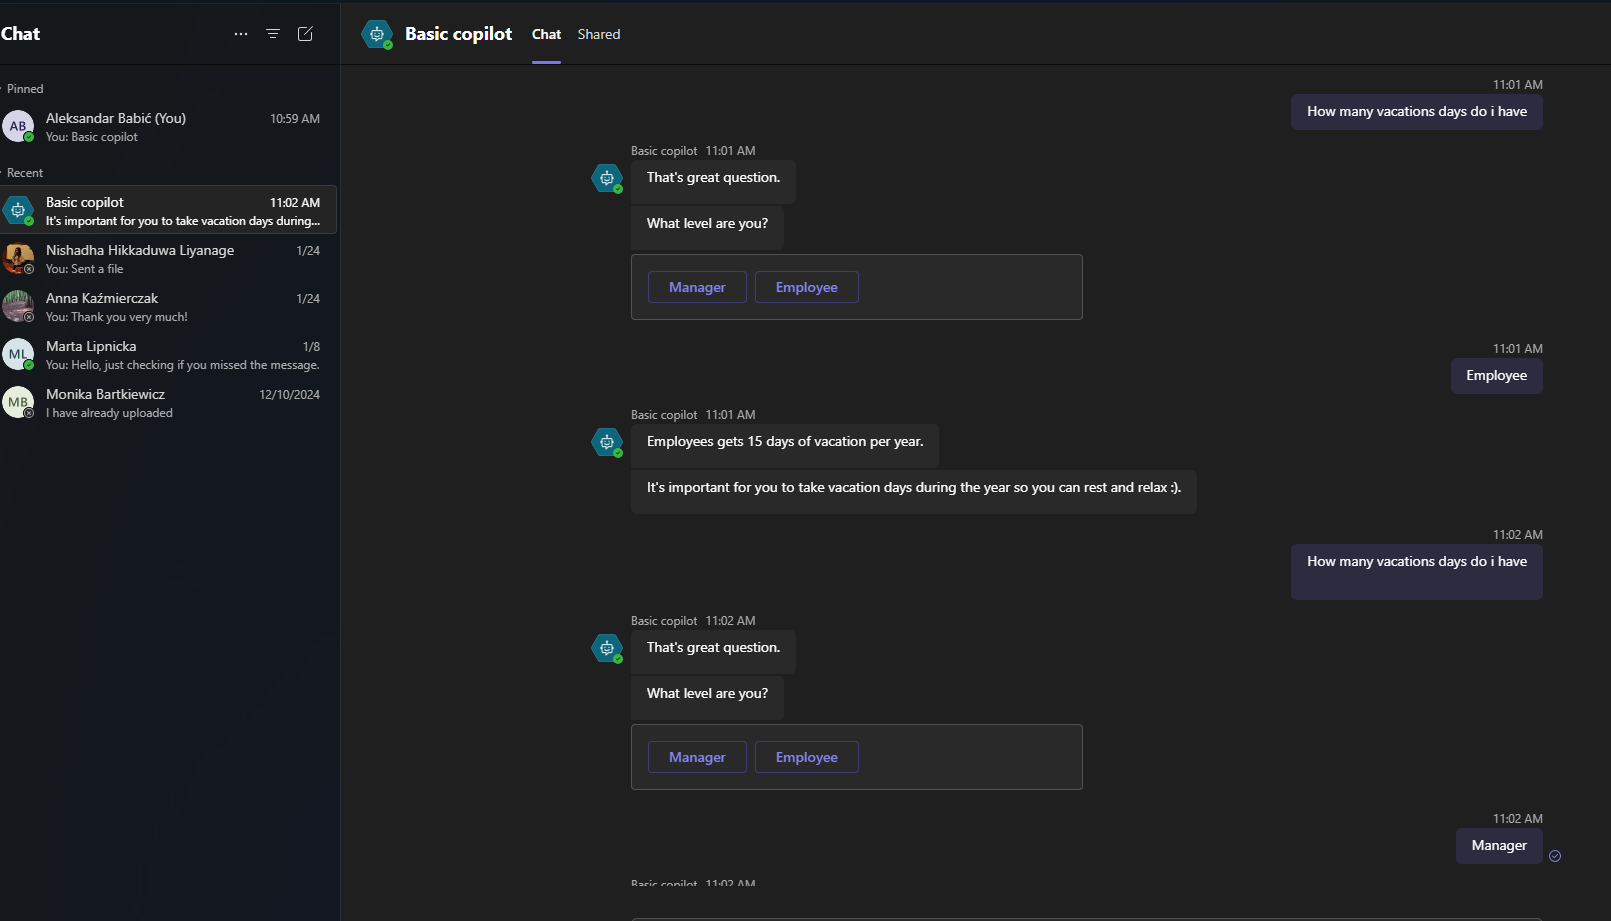
\includegraphics[width=0.6\textwidth]{./assets/Primjer_agenta_kreiranog_u_Copilot_Studiu.png} 
    \caption{Primjer agenta kreiranog u Microsoft Copilot Studiu}
    \label{fig:slika2}
\end{figure}

Osim toga isproban je i Bing Custom Search koji je vanjski servis koji se može koristiti za navođenje više izvora koji se koriste za odgovaranje na upite. Cilj je da se ne koristi cijeli
internet nego da se koristi taj skup podataka koji je naveden. Putem custom configuration ID-a može se povezati Custom Bing Search i Copilot Studio.
Naknadno isprobana je funkcionalnost Adaptive Cards Designer koji omogućava kreiranje vlastitih UI (eng. User Interface) elemenata koji se mogu koristiti unutar razgovora s korisnikom. 
Na sljedećoj slici može se vidjeti da je to JSON koji je potrebno importati u Copilot Studio. Na stranici \underline{https://adaptivecards.io/designer/} postoji veliki broj 
primjera koji su već kreirani i besplatni su za korištenje.

\begin{figure}[ht!]
    \centering
    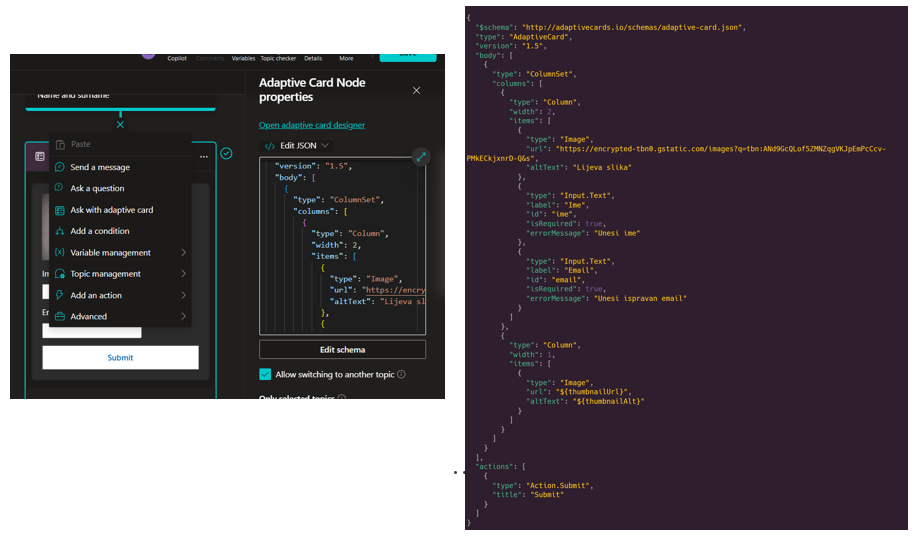
\includegraphics[width=0.7\textwidth]{./assets/Adaptive_cards.png} 
    \caption{Adaptive cards}
    \label{fig:slika3}
\end{figure}

Od drugih stvari koje još postoje u Copilot Studiju:
\begin{itemize}
\item dvije vrste kreiranje entiteta (Copilot sadrži veliki broj entiteta koji se mogu koristiti ali se mogu kreirati i vlastiti (Closed List i Regular Expression)),
\item message variation koji omogućava postojanje nekoliko verzija incijalnih poruka koje se pojavljuju kada se agent pokrene. 
\end{itemize}

\subsection{Agent}

AI agenti predstavljaju vrhunac automatizacije i autonomije jer su sposobni samostalno donositi odluke i poduzimati radnje bez stalnog ljudskog vodstva. Dizajnirani su za složena okruženja a 
također se dinamički prilagođavaju kako bi postigli definirane ciljeve. Djeluju samostalno kako bi analizirali podatke i odredili prioritetne zadatke. Prate sustave i okruženja, predviđaju i rješavaju 
potencijalne probleme prije nego što eskaliraju. Pri radu s složenijim problemima, identificiraju optimalnija rješenja. Bankarski agenti zamrzavaju kompromitirane račune kada se otkrije neovlašteni pristup s visokorizične lokacije.
Na primjer, prate stanje servera, otkrivaju anomalije, identificiraju kašnjenje pošiljka i proaktivno obavještavaju kupca nudeći naknadu ili alternative i poduzimaju korektivne mjere bez ljudske intervencije \cite{exomindset2025difference}.

\subsubsection{ChatGPT Operator}
ChatGPT Operator je agent koji može ići na web kako bi obavljao zadatke umjesto korisnika. Može pregledavati web stranicu i komunicirati s njom tipkanjem, klikanjem i pomicanjem.
Izašao je u siječnju 2025. godine i trenutno je još u fazi razvoja gdje se nastoji poboljšat rješenje na temelju povratnih informacija korisnika. Od Operatora se može zatražiti da obavi
širok raspon repetitivnih zadataka u pregledniku, kao što je ispunjavanje formi, naručivanje proizvoda, pa čak i stvaranje memeova. Operator je dostupan unutar PRO verzije na području SAD-a i pokreće se
na temelju modela CUA (eng. Computer-Using Agent). CUA je obučen za interakciju s grafičkim korisničkim sučeljima (eng. GUI) - gumbima, izbornicima i tekstualnim poljima koje ljudi vide na zaslonu.
Ako se dogodi se Operator susretne s izazovima ili ako napravi pogreške, u tom slučaju vraća kontrolu korisniku, osiguravajući glatko i korisničko iskustvo \cite{openai2024operator}. 

U nastavku se navodi jedan primjer koji ChatGPT Operator obavlja:
\begin{enumerate}
    \item Upravlja preglednikom i obavlja radnje u ime korisnika.
    \item Analizira podatke na temelju YouTube veze.
    \item Generira PNG sliku analize.
    \item Ide na X.com, lokalno odabire sliku i prenosi je.
    \item Lajka i komentira sliku.
    \item Često traži potvrdu prije izvođenja radnji.
    \item Može se koristiti za pretraživanje weba, kupnju ulaznica ili rezervaciju restorana.
\end{enumerate}
\newpage

\subsubsection{Manus}

Manus je višeagentni sustav koji se pokreće na temelju više modela. U Youtube videu \cite{manus} se može vidjeti snaga sustava kroz dva primjera:
\begin{itemize}
    \item Intervjuiranje - Dan mu je zip koji sadrži dosta životopisa (organizirane informacije). Uputa je da na temelju prošlog iskustva kandidata rangira kandidate i to zapiše na izvještaju.
    \item Pretraživanje - Traženje mjesta za stanovanje na temelju kriterija kao što je  sigurnost, kvaliteta škola i cijena. Na kraju je kreirao izvještaj.
\end{itemize}

Prilikom gledanja videa primijećen je komentar duhovitog karaktera, čijom je porukom istaknuto da je trenutno prisutan velik broj rješenjea u području umjetne inteligencije, pri čemu se 
kreativnost i inovativnost smatraju presudnim čimbenicima. 

\begin{figure}[ht!]
    \centering
    
\includegraphics[width=0.8\textwidth]{./assets/Manus_comment.png} 
    \caption{Manus komentar}
    \label{fig:slika4}
\end{figure}


\subsection{Chatbot}

Chatbotovi su sustavi temeljeni na kreiranim pravilima koji su osmišljena za izvršavanje određenih zadataka putem unaprijed definirane interakcije. Iako posjeduju dosta ograničenja jako se dobro
i brzo snalaze u dosljednom rješavanju jednostavnih repetativnih zadataka. Djeluju na temelju stabla odlučivanja ili prepoznavanja ključnih riječi ograničavajući svoju interakciju na unaprijed 
postavljene scenarije. Koriste se za automatizaciju zadataka gdje se obrađuje veliki broj ponavljajućih upita poput rezervacija ili narudžbi. Njihova mana je da se ne mogu prilagoditi izvan
svog programiranja što ih čini neprikladnim za složenije zadatke \cite{exomindset2025difference}.

\section{Inteligentni asistenti u obrazovnom sustavu}

Današnje obrazovanje se sve više oslanja na tehnologiju, a inteligentni asistenti postaju alat koji može poboljšati iskustvo učenja i poučavanja. Na primjer, svaki učenik može imati
personaliziranu pomoć, a učitelji imaju više vremena za fokusiranje na ono što je zaista važno. Takvi asistenti mogu prilagođavati materijale, odgovarati na pitanja, ocjenjivati domaće zadaće
čime se rasterećuje profesore. Jedna od najvećih prednosti koje donose inteligentni asistenti je personalizirano učenje. Umjesto univerzalnog pristupa, asistenti se mogu individualno 
posvetiti svakom učeniku/studentu. 

\subsection{Primjena inteligentnih asistenata u obrazovanju}

    \textbf{Automatizacija procesa ocjenjivanja} - ocjenjivanje pismenih zadataka, pružajući detaljne povratne informacije u roku od nekoliko minuta umjesto dana. 
    Osim što skraćuje vrijeme ocjenjivanja profesorima, učenici dobivaju brže povratne informacije o svom radu. Jedan od primjera je \href{https://www.gradescope.com/}{\underline{Gradescope}} kojeg je razvio Turnitin. 
    Kroz Gradescope moguće je ocjenjivati zadatke iz različitih predmeta, uključujući programiranje, fiziku, matematiku, kemiju, biologiju i ekonomiju. Također moguće je ocjenjivati
    programske projekte (u digitalnom obliku) i zadatke napisane na papiru. Neki od komentara profesora koji su koristili Gradescope su \cite{gradescope2025}:  
    \begin{itemize}
        \item "S Gradescopom je čast ocjenjivati. Prije što sam radio u rasponu od 2 do 3 sata sada odradim u 15 minuta" - Romulo Chumacero - University of Chile
        \item "Statistika mi stvarno pomaže da shvatim što sljedeći put mogu drugačije objasniti kako bih pomogla svojim učenicima da bolje uče" - Katie Johnson - Florida Gulf Coast University
        \item "Gradescope omogućuje da svaki dan svojoj grupi od 60 učenika dam kratki kviz i da ih sve ocijenim tijekom 30-minutne vožnje vlakom kući." -  Jesse Tov - Nortwestern University
    \end{itemize}

    \begin{figure}[ht!]
    \centering
    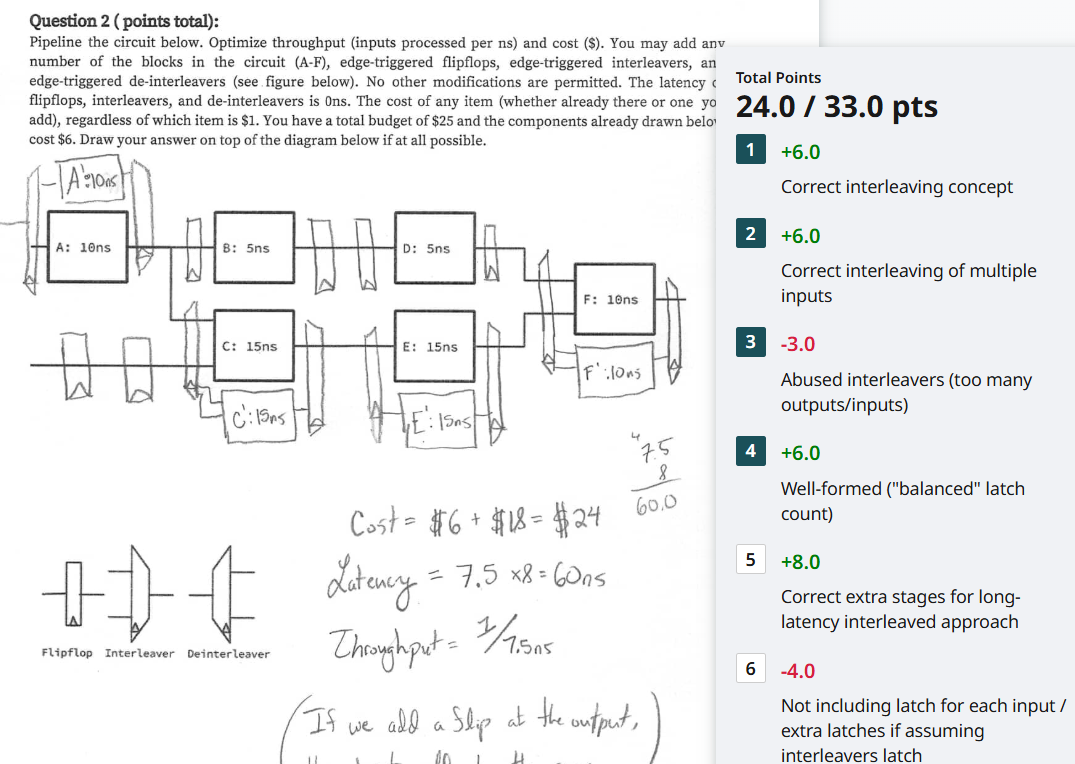
\includegraphics[width=0.8\textwidth]{./assets/Gradescope.png} 
    \caption{Ocjenjivanje zadatka - Gradescope}
    \label{fig:slika7}
    \end{figure}

    \textbf{Smanjenje adminstrativnog opterećenja} - na primjer, sustavi pokretani umjetnom inteligencijom mogu pratiti prisutnost, upravljati zadacima pa čak i predviđati kojim
    studentima je potrebna dodatna pomoć. Takav pristup pomaže u otkrivanju problema prije nego što postane još veći problem. Jedan od zanimljivijih citata od Rose Luckin, profesorice dizajna
    usmjerenog na učenike na University College London, je: "Prava moć inteligentnih agenata u obrazovanju ne leži u zamjeni učitelja, već u pojačavanju njihovog utjecaja. Obavljanjem rutinskih
    zadataka, AI assistenti oslobađaju edukatore da se usredotoče na ljudske elemente poučavanja, inspiraciju, mentorstvo i njegovanje vještina kritičkog razmišljanja" \cite{weber2025smythos}. 
    
    
    \textbf{Prilagođavanje nastavnih materijala}   - analiziranje snaga, slabosti i načina učenja svakog učenika kako bi se stvorili prilagođeni materijali. Na primjer, ako postoji
    učenik koji se muči s razlomcima, asistent može pružiti dodatne resurse kako bi se poboljšalo njegovo razumijevanje \cite{weber2025smythos}.


\subsection{Izazovi inteligentnih asistenata u obrazovanju}

Jedan od najvećih izazova je pitanje privatnosti podataka. Ovakvi sustavi zahtijevaju ogromne količine podataka o studentima da bi učinkovito funkcionirali, što ukazuje na opasnost od 
potencijalne zlouporabe tih podataka. Na primjer, studija Svučilišta u Michiganu iz 2020. godine otkrila je da 86 posto obrazovnih aplikacija umjetne inteligencije prikuplja osobne podatke od studenta,
a samo 42 posto ima jasne politike privatnosti \cite{weber2025smythos}.

Asistenti su dobri onoliko koliko su dobri podaci na kojima su obučeni. U obrazovnom sustavu, osiguranje kvalitete i relevantnosti tih podataka je od najveće važnosti.
Kako bi rješenje bilo zadovoljavajuće škole i programeri moraju surađivati kako bi stvorili sustave koji su ne samo učinkoviti, već i etični i sigurni \cite{weber2025smythos}.

Implementacija inteligentnih asistenata zahtijeva značajnu tehnološku infrastrukturu. Mnoge škole, posebno u ruralnim područjima, nemaju potreban hardver, brzi internet ili softver za podršku ovim sustavima.
Izvješće za obrazovanje iz 2022. godine kaže da gotovo 17 milijuna učenika u SAD-u još uvijek nema pristup internetu kod kuće \cite{weber2025smythos}.

Unatoč tim izazovima, integracija inteligentnih asistenata u obrazovni sustav donosi brojne prednosti. Sustavi pokretani umjetnom inteligencijom mogu automatizirati dugotrajne administrativne
zadatke, oslobađajući učitelje da se usredotoče na ono što najbolje rade: inspiriranje i poučavanje učenika. Osim toga, AI asistentni mogu pružiti personalizirano učenje, povećanu produktivnost
i učinkovitost, te poboljšano korisničko iskustvo \cite{weber2025smythos}.

Kroz sljedeće poglavlje je prikazano kako funkcioniraju inteligentni asistentni temeljeni na RAG (eng. Retrieval-Augmented generation) tehnologiji.
\newpage
\section{Retrieval Augmented Generation (RAG) metoda}

RAG je proces optimizacije izlaza velikog jezičnog modela pri čemu se referencira na autoritativnu bazu znanja izvan izvora podataka za obuku 
prije generiranje odgovora. Veliki jezični modeli (eng. Large Language Models - LLM) obučavaju se na ogromnim količinama podataka i koriste milijarde parametara za 
generiranje izlaza za zadatke poput odgovaranja pitanja, prevođenja jezika i dovršavanja rečenica. Ideja RAG-a je da proširi već moćne mogućnosti 
LLM-ova na određene specifične domene, a sve to bez potrebe za ponovnom obukom modela. Takav pristup poboljšava LLM-ove u smislu točnosti, 
korisnosti i relevantnosti \cite{awsRAG2025}.

Model velikog jezika može se zamisliti kao entuzijastičnog zaposlenika koji odbija biti informiran o aktualnim događajima, ali uvijek odgovara
na pitanja s visokim samopouzdanjem. Nažalost, takav stav može negativno utjecati na povjerenje korisnika i nije nešto što bi trebalo postojati
kod chatbotova. Iz takvih razloga RAG tehnologija preusmjerava LLM kako bi dohvatio relevantne informacije iz unaprijed definiranih izvora znanja \cite{awsRAG2025}.

Bez RAG-a, LLM uzima korisnički unos i stvara odgovor na temelju informacija na kojima je obučen. S RAG-om se uvodi komponenta za pronalaženje 
informacija koja koristi korisnički unos kako bi prvo privukla informacije iz novog izvora podataka. Nakon toga LLM kombinira novo znanje i svoje 
podatke za stvaranje boljih odgovora \cite{awsRAG2025}.

LLM-ovi su ključna tehnologija umjetne inteligencije koja pokreće chatbotove. Priroda LLM-ova je takva da ponekad unose dozu nepredvidljivosti
u generiranje odgovora. Osim toga, podaci o LLM obuci su statični i imaju krajnji rok za znanje koje posjeduju. Negativne strane LLM-ova uključuju \cite{awsRAG2025}:

\begin{itemize}
    \item iznošenje lažnih informacija kada na njih nema odgovora (nepoželjni efekti nazvani - halucinacijama), 
    \item prikazivanje zastarjelih informacija kada korisnik očekuje aktualan odgovor,
    \item izrada odgovora iz neautoriziranih izvora,
    \item stvaranje netočnih odgovora zbog terminološke zbrke, različiti izvori obuke koriste istu terminologiju za opisivanje različite stvari.
\end{itemize}

Veliki jezični modeli mogu biti nekonzistentni što bi značilo da ponekad točno odgovore na pitanja, a drugi put nasumično pogađaju. Ako povremeno zvuče kao da nemaju pojma što govore, 
to je zato što ustvari nemaju pojma. LLM znaju kako se riječi statistički povezivaju, ali ne znaju značenje riječi kao ni cjelinu njih poznatu kao rečenica. RAG također smanjuje potrebu 
korisnika da kontinuirano treniraju model na novim podacima i ažuriraju njegove parametre. Na taj način, RAG može smanjiti računalne i financijske troškove pokretanja chatbotova \cite{ibmRAG}.

\newpage

\begin{figure}[ht!]
    \centering
    \includegraphics[width=0.8\textwidth]{./assets/Konceptualni_tok_korištenja_RAG-a_s_LLM-ovima.jpg} 
    \caption{Konceptualni tok korištenja RAG-a s LLM-ovima \cite{awsRAG2025}}
    \label{fig:slika1}
\end{figure}

Funkcioniranje prikazanog sustava na slici \ref{fig:slika1}. opisano je kroz nekoliko  koraka \cite{awsRAG2025}:


\begin{enumerate}
    \item \textbf{Stvaranje vanjskih podataka} - novi podaci izvan orginalnog skupa podataka koji su se koristili za treniranje LLM-a se zovu 
    vanjski podaci (eng. external data). Oni dolaze iz više izvora podataka kao što su: API-ji ili baze podataka. Podaci mogu postojati u različitim formatima.
    Jedna od tehnika (eng. embeeding language models) pretvara podatke u numerički oblik i sprema ih u vektorsku bazu podataka 
    (kako bi generativni modeli umjetne inteligencije to mogli razumjeti).
    \item \textbf{Preuzimanje relevantnih informacija} - Korisnički upit pretvara se u vektorski prikaz i uspoređuje se s vektorskim bazama podataka.
    Na primjer, ako korisnik postavi pitanje chatbotu "Koliko dana godišnjeg odmora imam?", chatbot će morati preuzeti dokumente o politici godišnjeg 
    odmora uz evidenciju prošlih odmora za pojedinog zaposlenika. Takvi dokumenti će biti vraćeni korisniku jer su relevantni za njegov upit.
    \item \textbf{Proširivanje LLM upita} - Zatim, RAG model proširuje korisnički upit dodavanjem relevantnih dohvaćenih podataka u kontekstu. 
    Prošireni upit omogućuje modelima velikih jezika generiranje točnih odgovora na korisničke upite.
    \item \textbf{Ažuriranje vanjskih podataka} - Vrlo je bitno održati ažurne informacije i to se može ostvariti automatiziranjem procesa u stvarnom vremenu ili periodičnoj obradi. 
\end{enumerate}

Primjerice, ako se postavi pitanje: "Koji planet u Sunčevom sustavu ima najviše mjeseca?", osoba može odgovoriti: "Odlično pitanje! Kao dijete sam volio astronomiju i pročitao sam članak o tome
- mislim da je to Jupiter s 88 mjeseca." Međutim, takav odgovor ima nekoliko problema: osoba ne navodi konkretan izvor, iako nastupa s visokim samopuzdanjem ("ja to znam, pročitao sam")
te informacija može bit zastarjela jer se temelji na sjećanju iz prošlosti \cite{ibm2023rag}.

Kada bi osoba rekla: "Idem prvo na NASA-inu stranicu i tamo ću potražit tu informaciju", tada bi traženje odgovora bilo temeljeno na provjerenom i ažurnom izvoru.
Nasuprot tome, LLM-ovi, poput GPT-a, često odgovaraju vrlo samouvjereno, primjerice: "Na temelju podataka na kojima sam treniran, odgovor je Jupiter."
Iako zvuči uvjerljivo, takav odgovor može biti netočan, a korisnik često nije svjestan ograničenja modela ni datuma do kojeg je model treniran. U ovom slučaju, točan odgovor 
zapravo može biti Saturn, koji trenutno ima 114 poznatih prirodnih satelita. Rješenje za ovaj problem je korištenje tzv. content store-a - spremišta znanja koje može sadržavati izvore poput
internetskih stranica, PDF dokumenta ili baza podataka. LLM tada prvo pristupa tom vanjskom spremištu informacija, pretražuje ga, identificira relevantne sadržaje i tek tada generira
odgovor na temelju tih aktualnih podataka. U RAG sustavu prompt se najčešće sastoji od tri dijela: instrukcija (što model treba učiniti), korisnikovog upita (pitanje ili zahtjeva) i informacija 
koje su dohvaćene iz content store-a \cite{ibm2023rag}.
%Generirani odgovor se generira samo onda kada je LLM retriveao s relevantnim informacijama i to kombiniro s korisnikovim upitom.

\begin{table}[ht!]
    \centering
    \caption{Prednosti RAG-a \cite{awsRAG2025}}
    \begin{tabular}{|>{\centering\arraybackslash}m{5cm}|>{\raggedright\arraybackslash}m{10cm}|}
      \hline
      \textbf{Prednost} & \textbf{Opis} \\
      \hline
      Isplativa implementacija & Razvoj chatbota započinje korištenjem temeljnog modela (eng. Foundation models). Temeljni modeli su obično dostupni putem API ključeva i obučeni su na širokom spektru generaliziranih i neoznačenih podataka. Računalni i financijski troškovi za treniranje takvih modela su jako visoki. \\
      \hline
      Trenutne informacije & Iako su izvorni podaci LLM-a relevantni za specifične potrebe, teško je održati relevantnost. RAG se može koristiti za izravno povezivanje LLM-a s feedovima društvenih medija, web stranicama s vijestima i samim time pružiti korisnicima najnovije informacije. \\
      \hline
      Povećano povjerenje korisnika & RAG omogućuje prikazivanje točnih informacija s navođenjem izvora ili citata. Korisnici također mogu pretraživati izvorne dokumente ako im je potrebno dodatno pojašnjenje. \\
      \hline
      Više kontrole za razvojne programere & Učinkovitije testiranje i poboljšavanje aplikacija. Kontroliranje i mijenjanje izvora informacija. Rješavanje i ispravljanje problema. \\
      \hline
    \end{tabular}
\end{table}

Još jedan primjer je situacija u kojoj Alice želi saznati koliko dana porodiljnog dopusta može dobiti. Chatbot koji ne koristi RAG odgovara veselo i netočno ”Uzmi koliko želiš”.
Politike o porodiljnom dopustu su složene i razlikuju se ovisno o državi u kojoj se boravi. U ovom slučaju, veliki jezični model (LLM), umjesto da prizna ograničenje u znanju odgovarajući
"Žao mi je, ne znam", generirao je frazu iz svog skupa za treniranje koristeći korisnički orijentiran, ali neutemeljen jezik \cite{ibmRAG}.

Temelj svih temeljnih modela je arhitektura umjetne inteligencije poznata kao transformator. Pretvaraju se hrpe sirovih podataka u komprimirani prikaz njihove osnovne strukture. 
Fino-podešavanje (eng. Fine-tuning) – daje modelu punu širinu znanja koja mu je potrebna za odgovaranje na vrlo specifična pitanja u kontekstu koji se stalno mijenja. Tijekom 2020. godine, 
Meta (tadašnji Facebook) je osmislila okvir pod imenom ”retrieval-augmented generation” kako bi se omogućio pristup informacijama koje nisu ”samo one nad kojima su trenirani modeli” \cite{ibmRAG}.

RAG se sastoji od dvije faze: pronalaženje i generiranje sadržaja. U fazi pronalaženja algoritmi traže relevantne informacije za korisnikov upit dok se u fazi generiranja generira tekst 
kako bi se odgovorilo na korisnički upit. U okruženju otvorene domene te činjenice uglavnom dolaze iz indeksiranih dokumenata na internetu. U okruženju zatvorene domene obično se koristi 
uži skup izvora radi dodatne sigurnosti i pouzdanosti. Prije LLM-a, agenti su kroz razgovor pratili ručni tijek dijaloga. Pretpostavljali su namjeru klijenta, dohvaćali tražene informacije 
i dostavljali odgovor za određeni scenarij. Za jednostavne upite, ova ručna metoda stabla odlučivanja funkcionirala je sasvim dobro. Problem takvog pristupa je da se je gubilo vrijeme na 
pisanje i predviđanje svakog pitanja koje bi korisnik mogao postaviti. U takvim slučajevima, ako tražena informacija nije definirana u dostupnim podacima, chatbot neće bit u mogućnosti 
pružiti relevantan odgovor\cite{ibmRAG}. 

Danas chatbotovi bazirani na LLM-ovima mogu dati korisnicima odgovore bez da ljudi pišu definirane skripte. Samim nadovezivanjem RAG-a na LLM-ove smanjuje se potreba za ponovnim obučavanjem 
modela na novim primjerima \cite{ibmRAG}. Upiti korisnika nisu uvijek jednostavni, mogu biti dvosmisleno formulirani, složeni ili mogu zahtijevati znanje koje model nema. U takvim uvjetima 
LLM-ovi su skloni izmišljanju stvari. Rod Lastra opisuje velike jezične model kao “Zamislite model kao pretjerano nestrpljivog mlađeg zaposlenika koji izbrblja odgovor prije nego što provjeri činjenice”
Lastra dodatno ističe važnost svjesnog upravljanja neizvjesnošću u odgovaranjum, navodeći: “Iskustvo nas uči da zastanemo i kažemo kada nešto ne znamo. LLM-ovi moraju biti eksplicitno obučeni da prepoznaju pitanja na koja ne mogu odgovoriti” \cite{ibmRAG}. 

Kod finog podešavanja može se namjestiti da LLM zastane i kaže da ne zna ali za to je potrebno tisuće primjera pitanja na koja se ne može odgovoriti. Vektorske baze podataka 
se mogu učinkovito indeksirati, pretraživati te je u njih jednostavno pohraniti veliku količinu informacija. RAG je još uvijek relativno nova tehnologija, a brojni izazovi vezani uz njezinu
pouzadnost i implementaciju još uvijek nisu u potpunosti riješeni \cite{ibmRAG}.


\chapter{React}

Svijet danas ne funkcionira bez mobilnih i web aplikacija. Sve se orijentira prema digitalizaciji, od rezerviranja hrane do naručivanja vožnje u taksiju. Vrlo je bitno napraviti vizualno
primamljivu aplikaciju a React je upravo jedna od popularnijih frontend biblioteka koja to omogućava. React je temeljen na JavaScriptu i široko se koristi u web razvoju. U usporedbi s drugim tehnologijama
, React je nova tehnologija, a osnovan je od strane Jordan Walkea 2011. godine (softverski inženjera u Facebooku). Reactova popularnost dolazi radi nekoliko razlog \cite{simplilearn2025react}:
\begin{itemize}
    \item jednostavno stvaranje dinamičkih aplikacija,
    \item korištenje Virtual DOM čime se aplikacije brže izrađuju (ažurira komponente samo koje su promijenjene),
    \item podjela na komponente - jedna aplikacija se sastoji od više komponenti koje se mogu koristit kroz cijelu aplikaciju (što smanjuje vrijeme razvoja aplikacije),
    \item mala krivulja učenja - React je jednostavan za učenje jer kombinira HTML i JavaScript koncepte,
    \item koristi se za razvoj web i mobilnih aplikacija - React Native - za mobilne aplikacije,
    \item jednostavno otklanjanje grešaka - Facebook je izdao Chromeovo proširenje koje se može koristit za otklanjanje pogrešaka u React aplikacijama.
\end{itemize}

\begin{figure}[ht!]
    \centering
    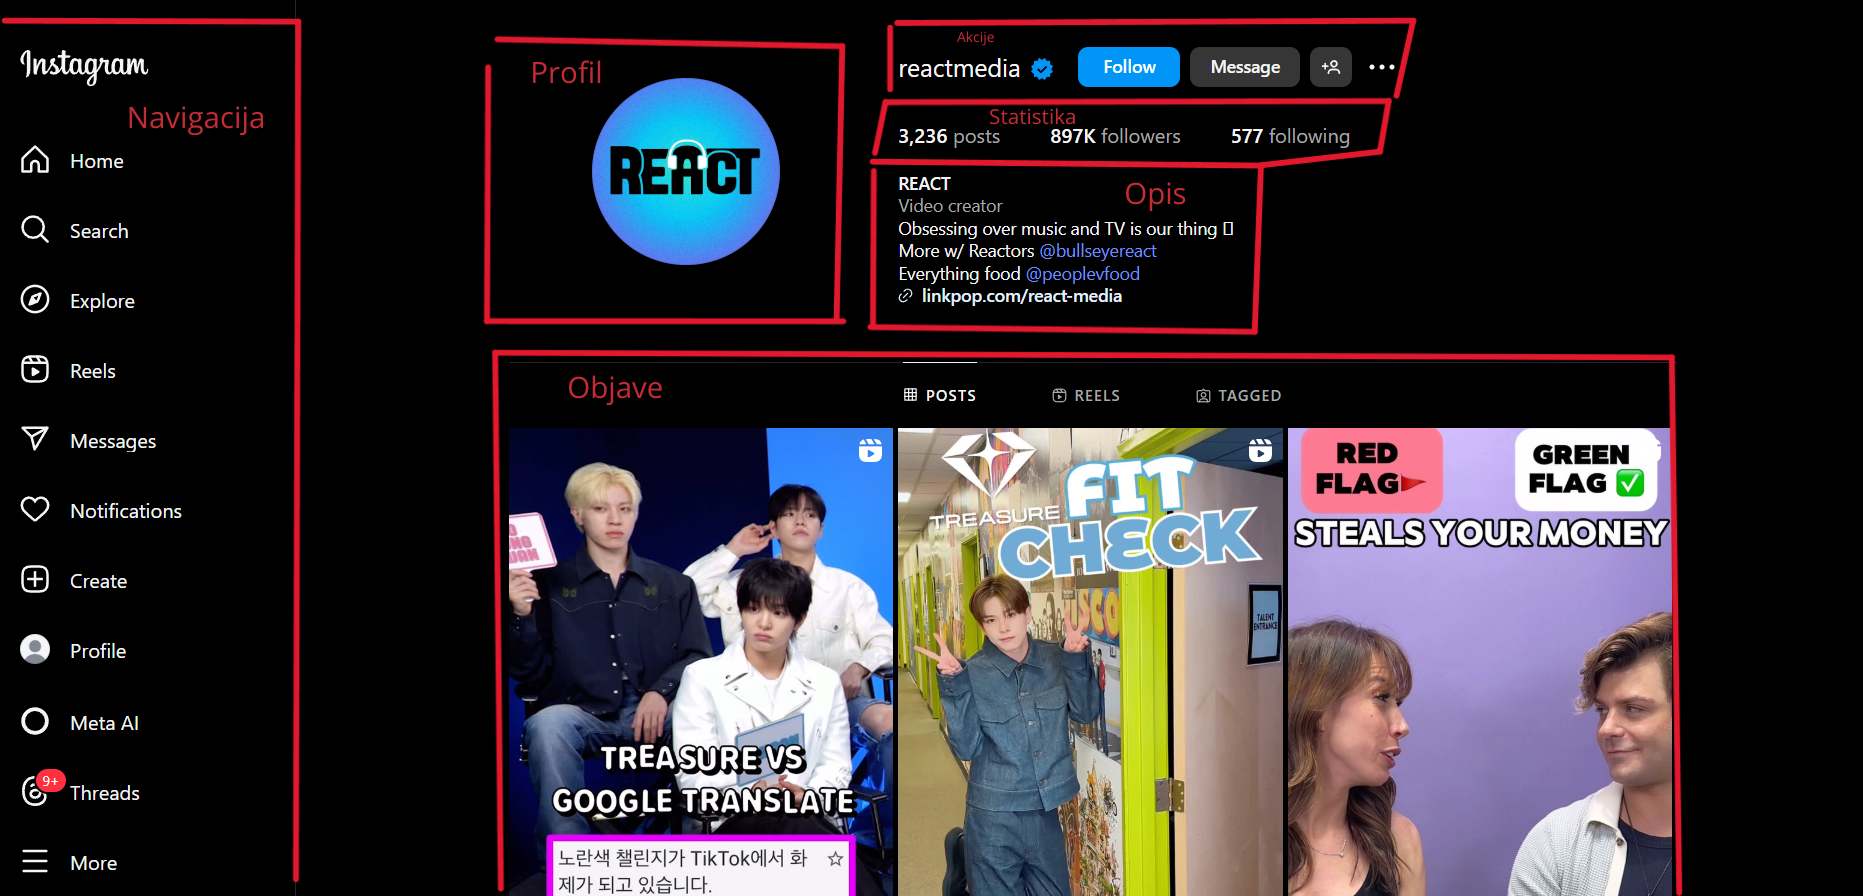
\includegraphics[width=0.6\textwidth]{./assets/components.png} 
    \caption{React komponenta}
    \label{fig:slika5}
\end{figure}


Jedna zanimljivost vezana uz React programere, promatrana na dvije potpuno različite lokacije, otkriva da su indijski developeri za isti posao plaćeni i do deset puta manje (podaci za 2021. godinu). 
To jasno odražava razliku u životnom standardu i ekonomskim potrebama pojedinih zemalja \cite{simplilearn2025react}.
\begin{itemize}
    \item Prosječna plaća za početnog React developera u SAD-u iznosi oko 87000 USD godišnje,
    \item Prosječna plaća za početnog React developera u Indiji iznosi oko 8000 USD godišnje.
\end{itemize}



\chapter{Praktični dio rada}
Praktični dio rada se sastoji od izrade web stranice i izrade inteligentnog asistenta temeljenog na RAG tehnologiji. Za izradu frontenda korišten je
JavaScript u Reactu. React predstavlja jedno od najpopularnijih frameworka za izradu web aplikacija. Posebno se ističe zbog toga što omogućava
razvoj aplikacija koje su brze, jednostavne i lako održive. Osim toga, najbitnija stvar je što React gradi aplikaciju po komponentama, što omogućava
jasnije razumijevanje koda kao i njegovo olakšano preuređivanje. Za izradu inteligentnog asistenta prvotno je napravljen scraper podataka s kojim je
izrađen skup podataka koji je poslužio za treniranje inteligentnog asistenta.

Backend je ...

Popis funkcionalnosti - napraviti tablicu možda.

\section{Izrada web stranice}

\begin{table}[h!]
    \centering
    \begin{tabular}{|l|p{7cm}|p{7cm}|}
    \hline
    \textbf{Stranica} & \textbf{Komponente} & \textbf{Opis} \\
    \hline
    Sve stranice & Header, Footer & Zajednički elementi svih stranica. \\
    \hline
    Početna & Slider, Motivacija, Kratko o Łódźu, Drugi gradovi & Linkovi prema drugim stranicama. \\
    \hline
    About \mbox{Łódź} & Dodatno o gradu, Review EX studenata & Informacije i iskustva studenata Erasmus+. \\
    \hline
    Other Cities &  & Pregled ostalih gradova Poljske. \\
    \hline
    Questions & Forma za pitanja & Ako asistent ne zna odgovor. \\
    \hline
    AI asistent & Sučelje za razgovor s korisnikom &  \\
    \hline
    \end{tabular}
    \caption{Struktura stranica i njihovih komponenti}
\end{table}

\section{Izrada inteligentnog asistenta}

\subsection{Prikupljanje podataka}
\subsection{Treniranje modela}
\subsection{Server}
\section{Prikaz rada aplikacije}




\chapter{Zaključak}



Za kraj, Erasmusa se ne treba bojati jer je to prekasno iskustvo koje se pamti do kraja života. Svaki problem s kojim se suoči osoba, čini osobu jačom i neovisnijom. 
Boravak na jednom mjestu dulje vrijeme postat će čudan način života. Jednom Erasmus+, uvijek Erasmus+!
Poveznica na Github: \href{https://github.com/ababic20/Website-with-a-chatbot.git}{\textbf{Poveznica}} 

\makebackmatter



\end{document}
